\documentclass[12pt]{article}

\usepackage[portuges]{babel} % Region format pt-br
\usepackage[latin9]{inputenc} % Caracteres e acentos
\usepackage{enumerate} % Listas
\usepackage{setspace} % Espa�amento de linha
\usepackage{color} % Cores no texto
\usepackage{graphicx} % Imagens
\usepackage{hyperref}
\usepackage{csquotes}
\usepackage{amsmath}
\usepackage{geometry}
\usepackage{listings}
\usepackage{subcaption}
\usepackage{placeins}
\usepackage{amssymb}
\usepackage[]{algorithm2e}
\usepackage{systeme}

%\documentclass[border=3mm]{standalone}
\usepackage{pgfplots}
\pgfplotsset{compat=1.13}


\geometry{a4paper,total={210mm,297mm},left=20mm,right=20mm,top=20mm,bottom=30mm,}
\graphicspath{ {imgs/} } % Path com imagens

\def\changemargin#1#2{\list{}{\rightmargin#2\leftmargin#1}\item[]} % Fun��o para mexer nas margens de paragrafos
\let\endchangemargin=\endlist 


\usepackage{color}

\definecolor{mygreen}{rgb}{0,0.6,0}
\definecolor{mygray}{rgb}{0.5,0.5,0.5}
\definecolor{mymauve}{rgb}{0.58,0,0.82}

\lstset{ %
	backgroundcolor=\color{white},   % choose the background color; you must add \usepackage{color} or \usepackage{xcolor}; should come as last argument
	basicstyle=\footnotesize,        % the size of the fonts that are used for the code
	breakatwhitespace=false,         % sets if automatic breaks should only happen at whitespace
	breaklines=true,                 % sets automatic line breaking
	captionpos=b,                    % sets the caption-position to bottom
	commentstyle=\color{mygreen},    % comment style
	deletekeywords={...},            % if you want to delete keywords from the given language
	escapeinside={\%*}{*)},          % if you want to add LaTeX within your code
	extendedchars=true,              % lets you use non-ASCII characters; for 8-bits encodings only, does not work with UTF-8
	frame=single,	                   % adds a frame around the code
	keepspaces=true,                 % keeps spaces in text, useful for keeping indentation of code (possibly needs columns=flexible)
	keywordstyle=\color{blue},       % keyword style
	language=Octave,                 % the language of the code
	morekeywords={*,...},            % if you want to add more keywords to the set
	numbers=left,                    % where to put the line-numbers; possible values are (none, left, right)
	numbersep=5pt,                   % how far the line-numbers are from the code
	numberstyle=\tiny\color{mygray}, % the style that is used for the line-numbers
	rulecolor=\color{black},         % if not set, the frame-color may be changed on line-breaks within not-black text (e.g. comments (green here))
	showspaces=false,                % show spaces everywhere adding particular underscores; it overrides 'showstringspaces'
	showstringspaces=false,          % underline spaces within strings only
	showtabs=false,                  % show tabs within strings adding particular underscores
	stepnumber=2,                    % the step between two line-numbers. If it's 1, each line will be numbered
	stringstyle=\color{mymauve},     % string literal style
	tabsize=2,	                   % sets default tabsize to 2 spaces
	title=\lstname                   % show the filename of files included with \lstinputlisting; also try caption instead of title
}


\begin{document}

%---------------------------------------------------------------------------------
%	Capa
%---------------------------------------------------------------------------------

\begin{titlepage}

\newcommand{\HRule}{\rule{\linewidth}{0.4mm}} % Defines a new command for the horizontal lines, change thickness here

\begin{center}

\begin{figure}[h]
	\centering
	\begin{subfigure}[b]{.1\linewidth}
		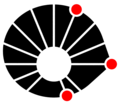
\includegraphics[width=\linewidth]{!-logo_unicamp}
	\end{subfigure}
	\begin{subfigure}[b]{.1\linewidth}
		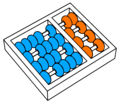
\includegraphics[width=\linewidth]{!-logo_ic}
	\end{subfigure}
\end{figure}

\textsc{\large Universidade Estadual de Campinas}\\[0.1cm]
\textsc{\normalsize Instituto de Computa��o}\\[3.5cm]
\textsc{\large MO644 - Introdu��o � Programa��o Paralela}

\HRule \\[0.2cm]

\setstretch{2}
{\Large \bfseries Tarefa 12}
\HRule \\[2cm]

\doublespacing

\begin{minipage}{0.5\textwidth}
\begin{flushleft} \normalsize
\emph{Student:} \par
192744,	Miguel Antonio Rodriguez Santander
\end{flushleft}
\end{minipage}
~
\begin{minipage}{0.45\textwidth}
\begin{flushright} \normalsize
\emph{Teacher:} \par
Guido Ara�jo
\end{flushright}
\end{minipage}\\[8cm]

{\large junho de 2017}\\[3cm]

\vfill

\end{center}
\end{titlepage}

%---------------------------------------------------------------------------------
%	Conte�do
%---------------------------------------------------------------------------------

\setlength{\parindent}{3em}
\setlength{\parskip}{0.7em}
\setstretch{1.3}
\setcounter{page}{1}
\setcounter{figure}{0}

\section{Introduction}
\label{sec:introduction}

This laboratory consisted in working with The OmpCloud tool, which , allows to mix the tools of OpenMP with Spark and the use of clusters in the cloud. This tool, allows to solve problems using distribuited clusters, very fast and efficient. For this we prepare a pair of experiments with the multiplication of two matrices, which have very large sizes, and the calculation becomes very expensive for even a simple computer.

\section{Programming and configuration}
\label{sec:programming}
In order to use OmpCloud\footnote{\href{https://ompcloud.github.io/}{https://ompcloud.github.io/}} in our code, it is necessary to use the OpenMP clauses that this tool has included. As we can see in the Listing~\ref{list:funcion_ompclud}, the first action was to map all variables that will be used in the cloud. Then for each  \textit{for} statement a parallelization is performed using the pragma of the \textit{for} statement, and within each for a unique OmpCloud statement is used, which allows data partitions to be partitioned in the map clauses. Whit this the cloud is responsible for making the calculation using Spark, which can be hosted inside the same computer where it is hosting, or can also be in some cloud like Microsoft Azure,\footnote{\href{https://azure.microsoft.com}{https://azure.microsoft.com}} or Amazon Web Services.\footnote{\href{https://aws.amazon.com/}{https://aws.amazon.com/}}.

\begin{lstlisting}[language=C, caption=Function used to calculate Matrix Multiplication with clausules of OmpCloud., label=list:funcion_ompclud, frame=single]
// Kernel to parallelize using OmpCloud
void mm2_OMP(float *A, float *B, float *C, float *D, float *E) {

	//Maping data to cloud
	#pragma omp target map(alloc: C[:N*N]) map(to: A[:N*N], B[:N*N], D[:N*N]) map(from: E[:N*N])  device(CLOUD)
	{
		//Paralleling for
		#pragma omp parallel for
		for (int i = 0; i < N; i++) {
			//Using clausule to split data into CLOUD.
			#pragma omp target data map(to: A[i*N:(i+1)*N]) map(from: C[i*N:(i+1)*N])
			for (int j = 0; j < N; j++) {
				C[i * N + j] = 0.0;
				for (int k = 0; k < N; ++k) {
					C[i * N + j] += A[i * N + k] * B[k * N + j];
				}
			}
		}
		
		//Paralleling for
		#pragma omp parallel for
		for (int i = 0; i < N; i++) {
			//Using clausule to split data into CLOUD.
			#pragma omp target data map(to: C[i*N:(i+1)*N]) map(from: E[i*N:(i+1)*N])
			for (int j = 0; j < N; j++) {
				E[i * N + j] = 0.0;
				for (int k = 0; k < N; ++k) {
					E[i * N + j] += C[i * N + k] * D[k * N + j];
				}
			}
		}
	}
}
\end{lstlisting}

For the case of this laboratory, the Microsoft Azure cloud tool was used, in which it was possible to create a cluster with Spark 2.0.1, which is named \textit{cluster192744-3}, it contains 40 cores, the which are dividen into 8 cores divided into two nodes, as Heads or masters. The other 32 cores in 4 nodes, named workers o slaves. In order to make the connection to this cluster, OpmCloud allows the configuration through a file shown in the Listing~\ref{list:configuracion}.

\begin{lstlisting}[caption=Configuration for contect to Azure., label=list:configuracion, frame=single]
[AzureProvider]
Cluster=cluster192744-3
StorageAccount=storages192744
StorageAccessKey=lX96y0fr2s/fmmU76KfK/r2OHUgNYJmkcwZXW0anuHhcEwbz+TAOQJXCPUxSpdJ/CS6dWalBl4sRsZcXEzYzow==

[Spark]
User=sshuser
WorkingDir=/home/sshuser/
\end{lstlisting}

\section{Experiments}
\label{sec:experiments}

To see how much better a cluster's performance than the serial version is, we set out to experiment with different sizes of matrices (100, 500, 1000, 1500, 2000). In Fig.~\ref{fig:speedup} we can see that as the value of $N$ increases, the speedup observed by the execution in the cloud is better, because when the value is very small, the overhead cost to send the data to the cluster, running it in different machines, is greater than executing the code in local machine.

In Fig~\ref{fig:metric:resumen} we ca observe the metrics obtained by the execution of each of the experiments, where it can be observed in detail that as the value of $N$ increases, the amount of time spent in the execution is greater for each core.


\begin{figure}
	\centering
\pgfplotstableread[row sep=\\,col sep=&]{
	interval & Local & Cloud \\
	100     & 0.1 & 46.56   \\
	500     & 1.14  & 50.34   \\
	1000     & 7.75 & 54.81  \\
	1500    & 30.14 & 67.38 \\
	2000   & 92.10 & 83.87\\
}\mydata

\begin{tikzpicture}
\begin{axis}[
ybar,
bar width=.9cm,
width=0.9\textwidth,
height=.5\textwidth,
legend style={at={(0.5,1)},
	anchor=north,legend columns=-1},
symbolic x coords={100,500,1000,1500,2000},
xtick=data,
nodes near coords,
nodes near coords align={vertical},
ymin=0,ymax=120,
ylabel={\Time (s)},
]
\addplot table[x=interval,y=Local]{\mydata};
\addplot table[x=interval,y=Cloud]{\mydata};
\legend{Local Time, Cloud Time}
\end{axis}
	\end{tikzpicture}
	\caption{Speedup with different sizes of the matrix.}
	\label{fig:speedup}
\end{figure}



\begin{figure}
	\centering
	\begin{subfigure}{0.47\textwidth}
		\centering
		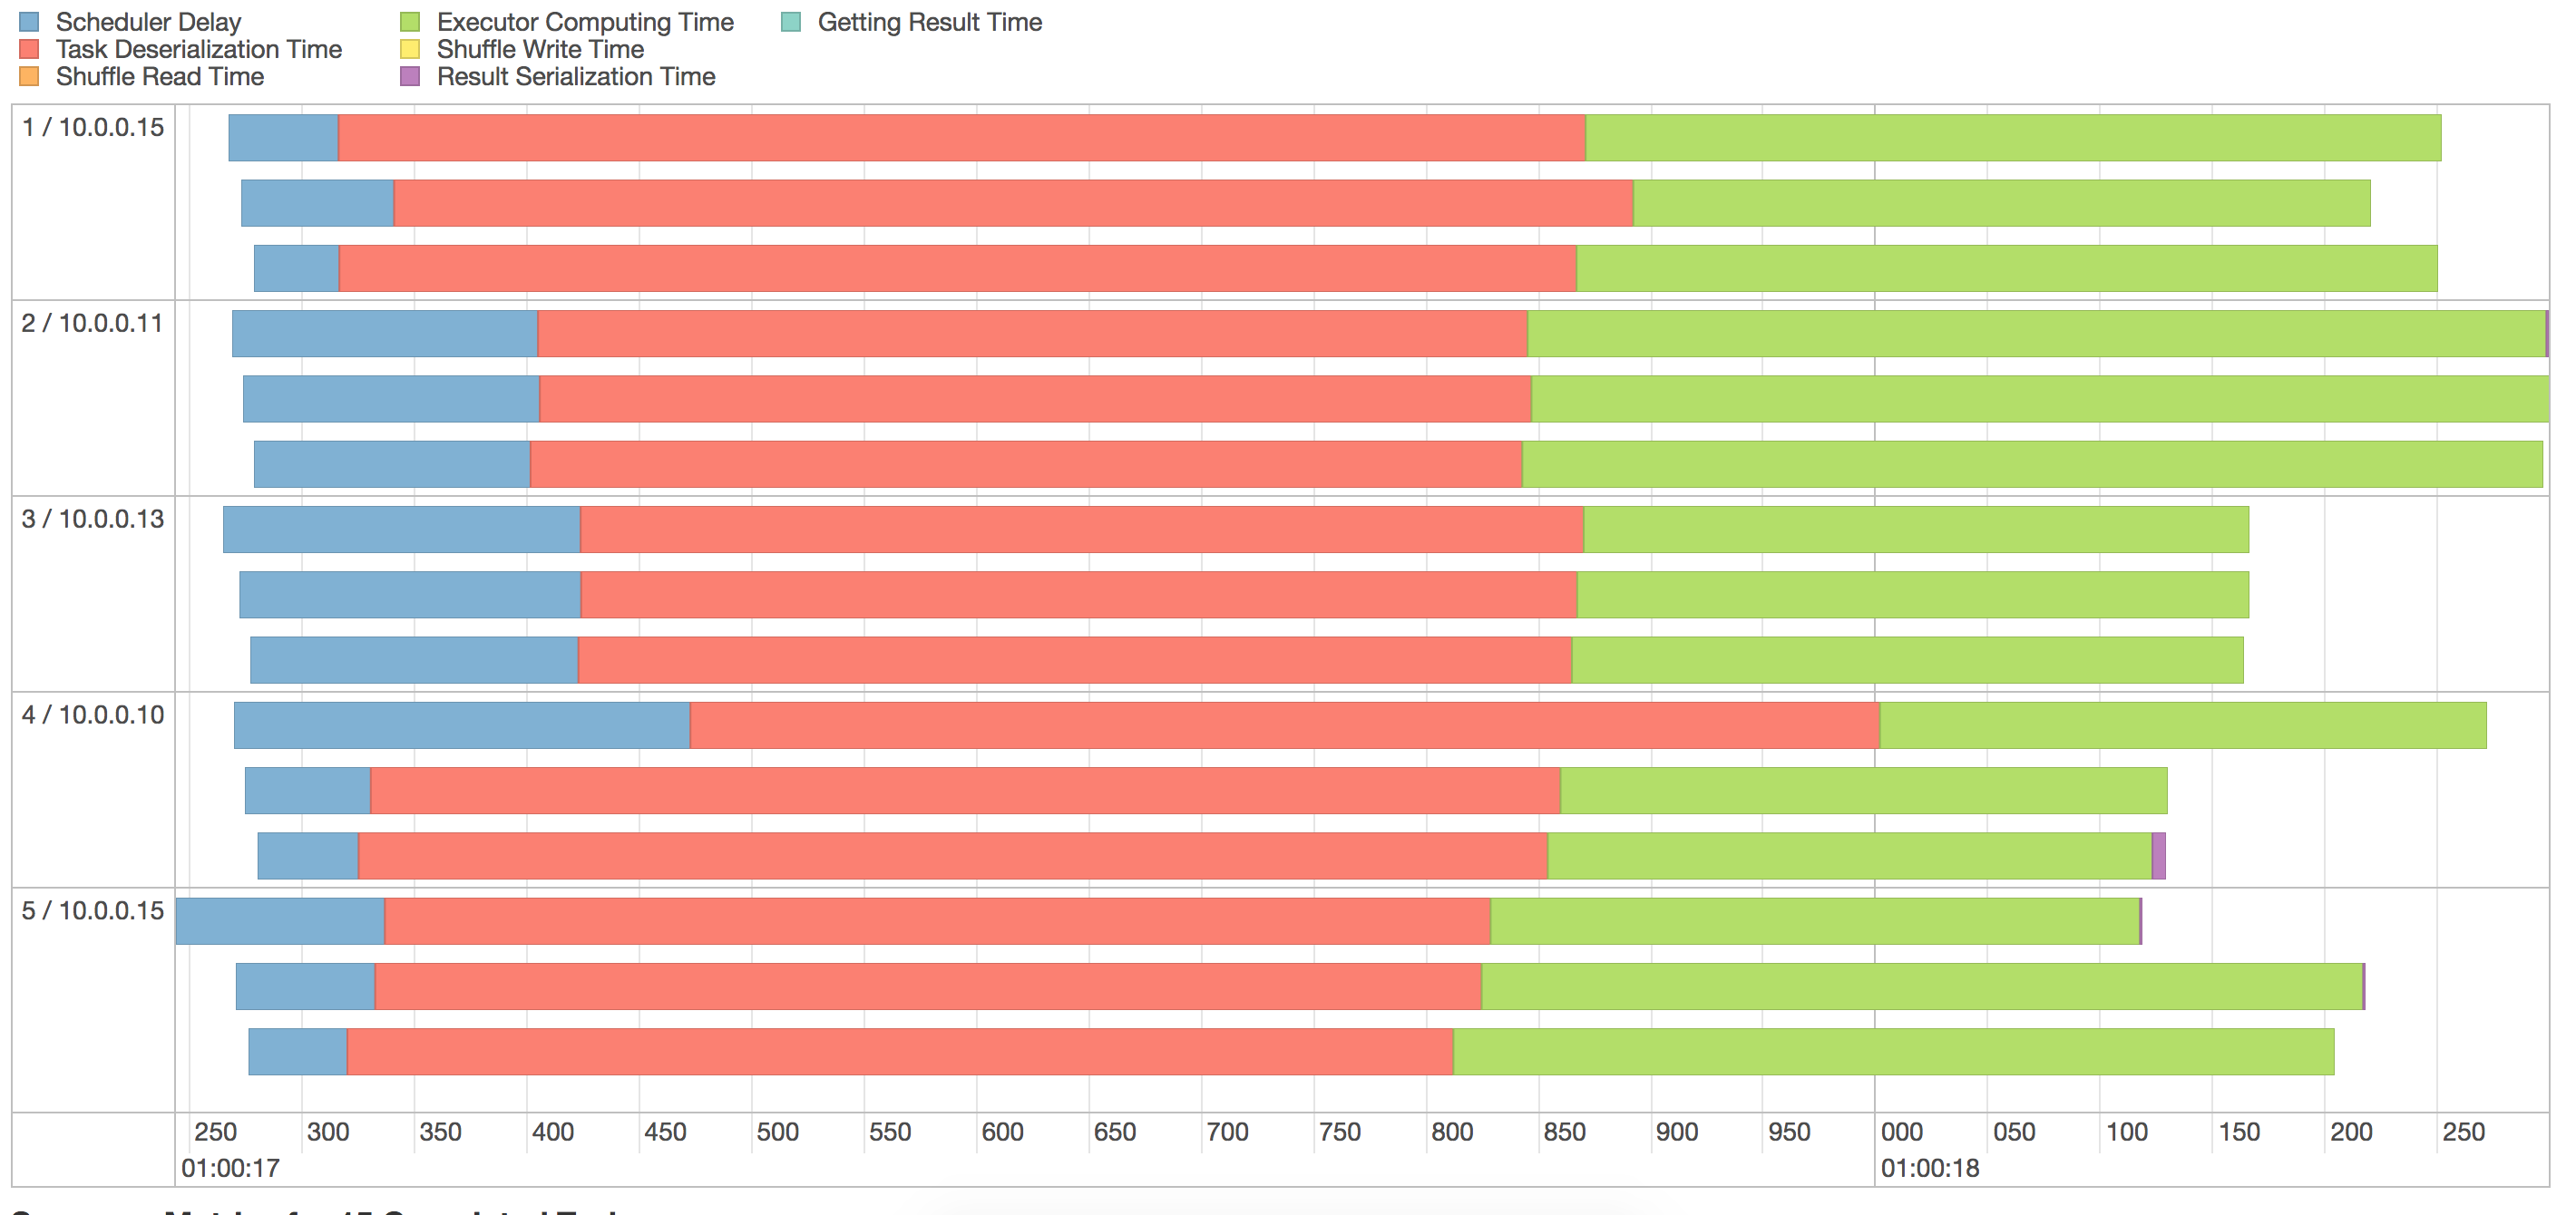
\includegraphics[width=1.0\linewidth]{n100} 
		\caption{Metric with $N=100$}
		\label{fig:metric:n100} 
	\end{subfigure}
	\centering
	\begin{subfigure}{0.47\textwidth}
		\centering
		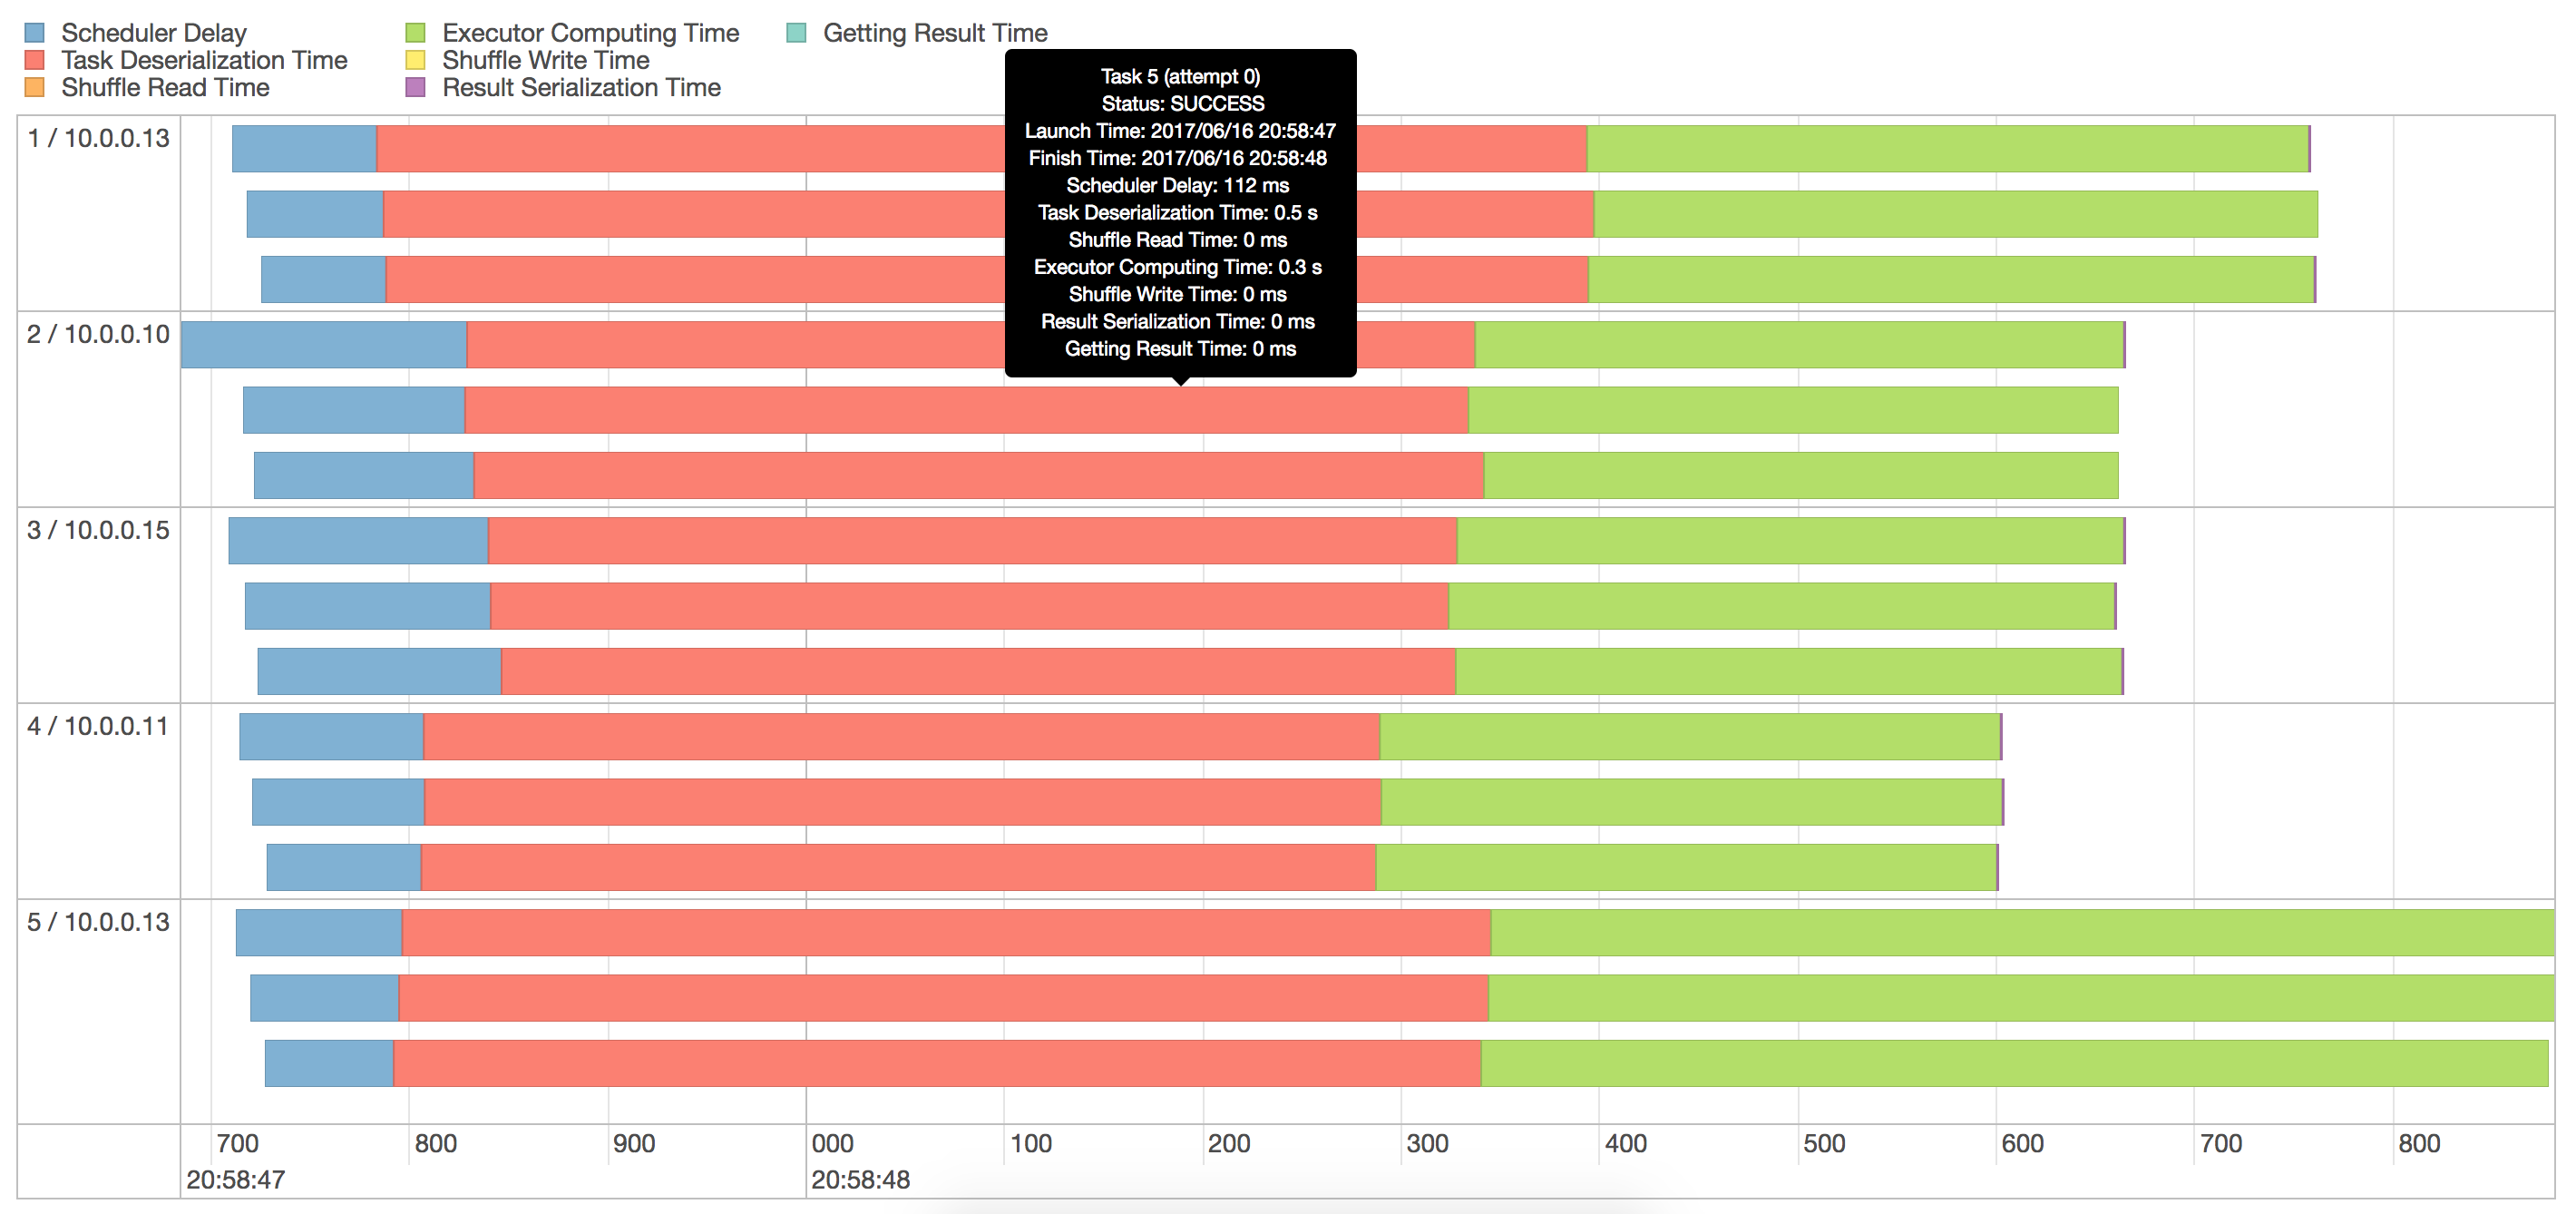
\includegraphics[width=1.0\linewidth]{n500}
		\caption{Metric with $N=500$}
		\label{fig:metric:n500}
	\end{subfigure}
	
	
	\centering
	\begin{subfigure}{0.90\textwidth}
		\centering
		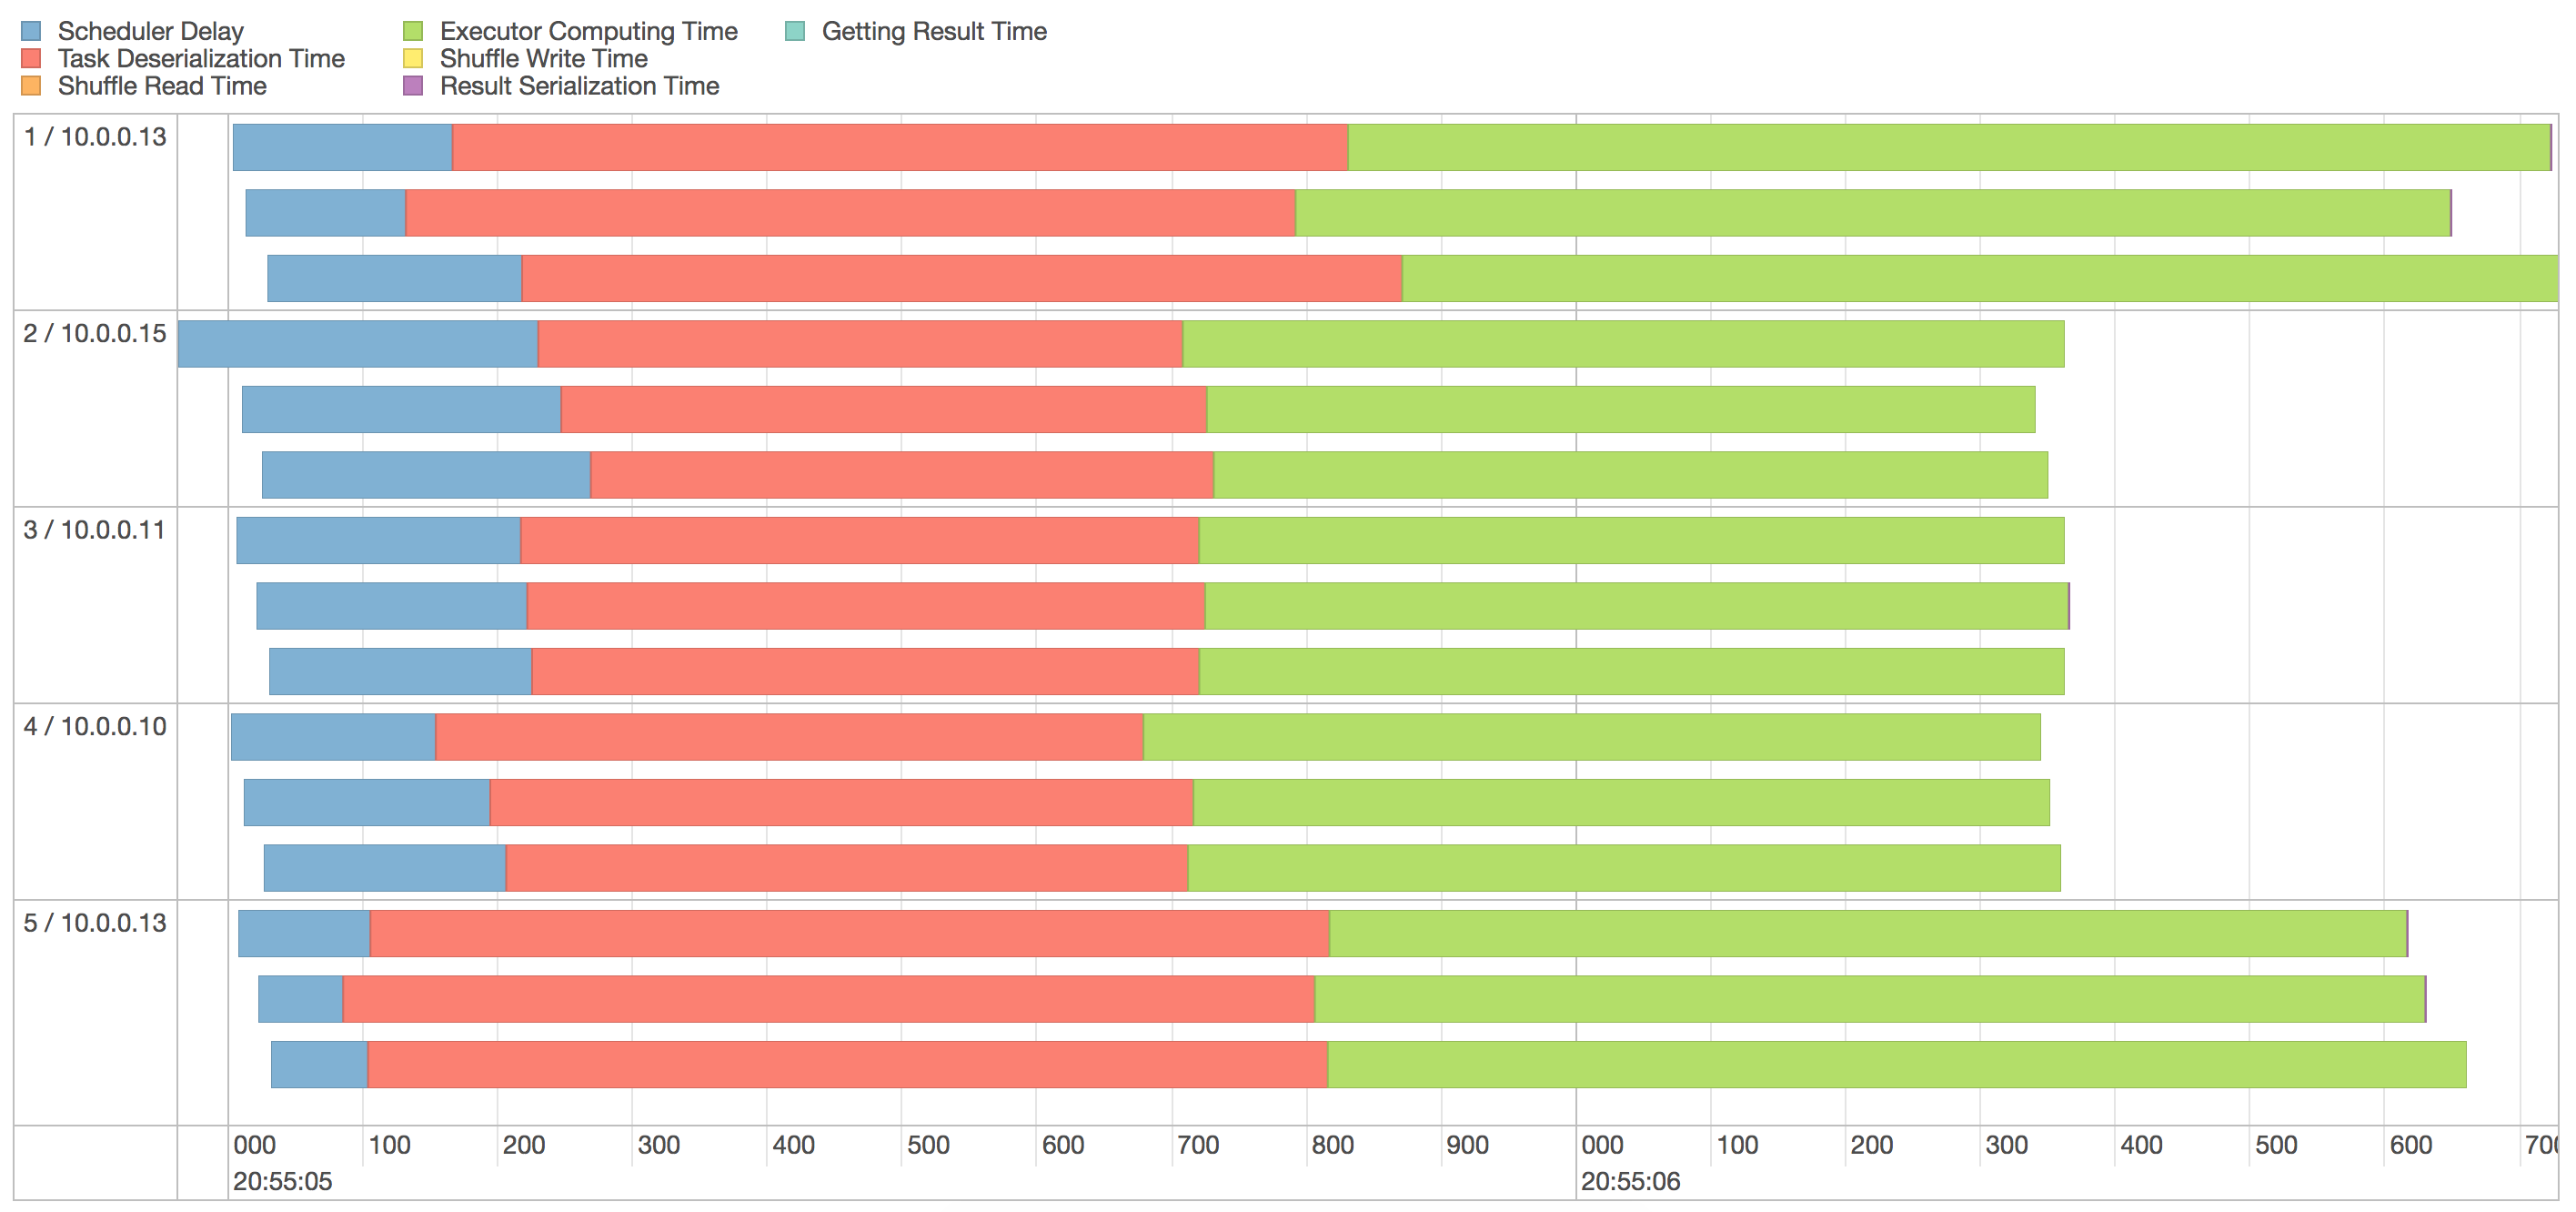
\includegraphics[width=1.0\linewidth]{n1000} 
		\caption{Metric with $N=100$}
		\label{fig:metric:n1000} 
	\end{subfigure}
	
	\centering
	\begin{subfigure}{0.47\textwidth}
		\centering
		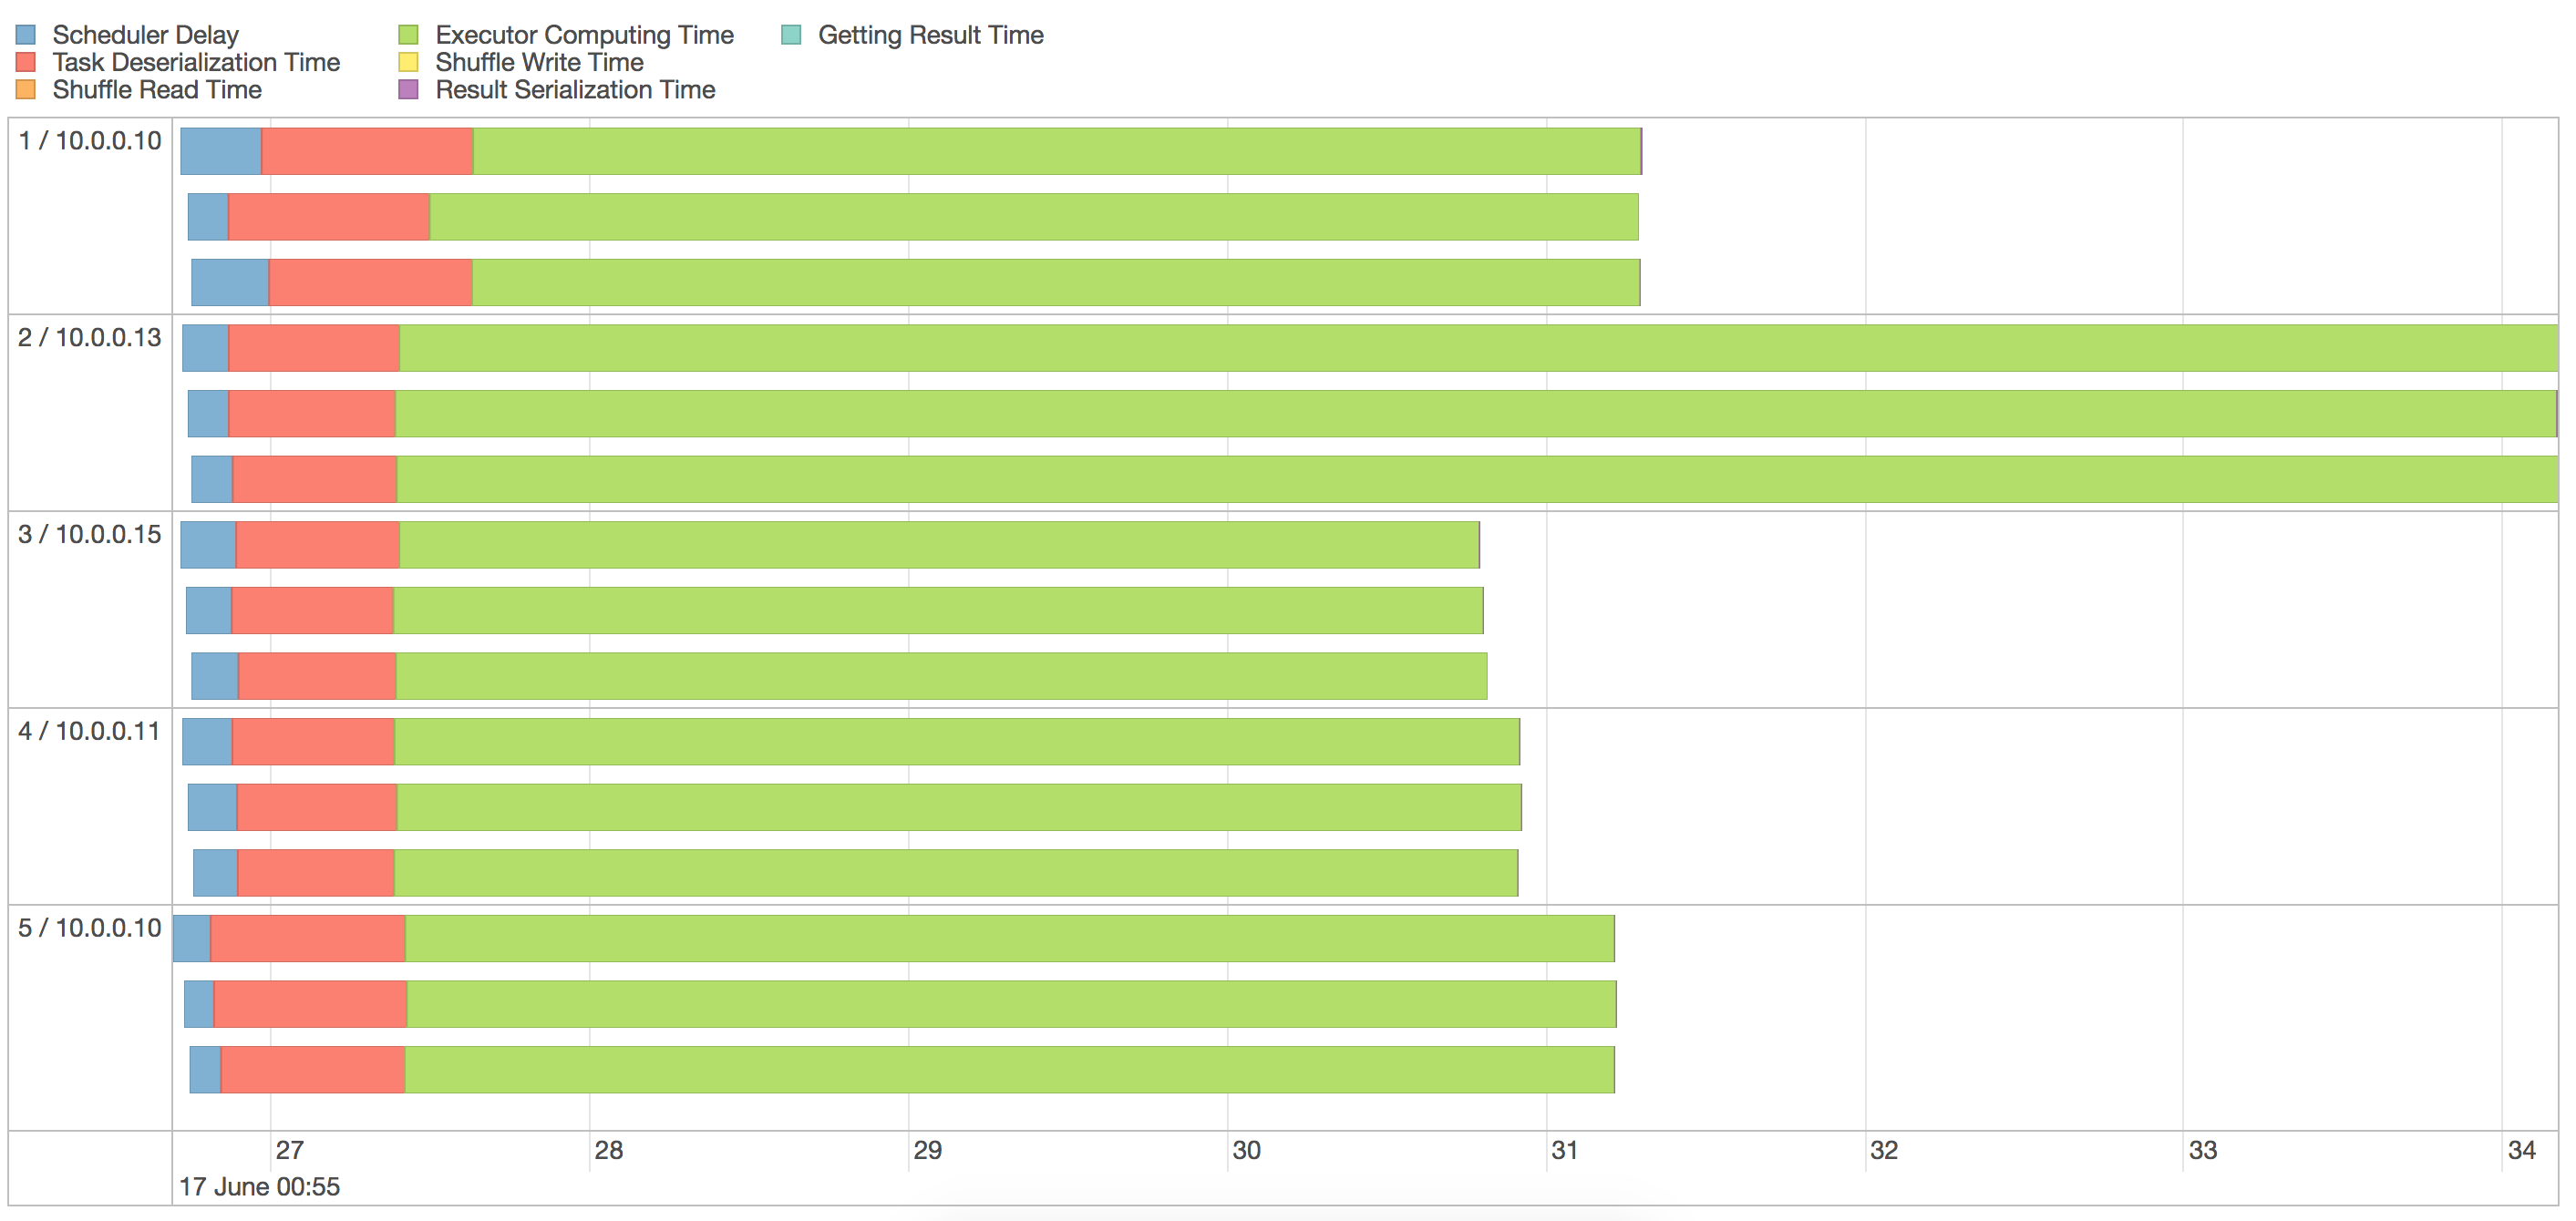
\includegraphics[width=1.0\linewidth]{n1500} 
		\caption{Metric with $N=1500$}
		\label{fig:metric:n1500} 
	\end{subfigure}
	\centering
	\begin{subfigure}{0.47\textwidth}
		\centering
		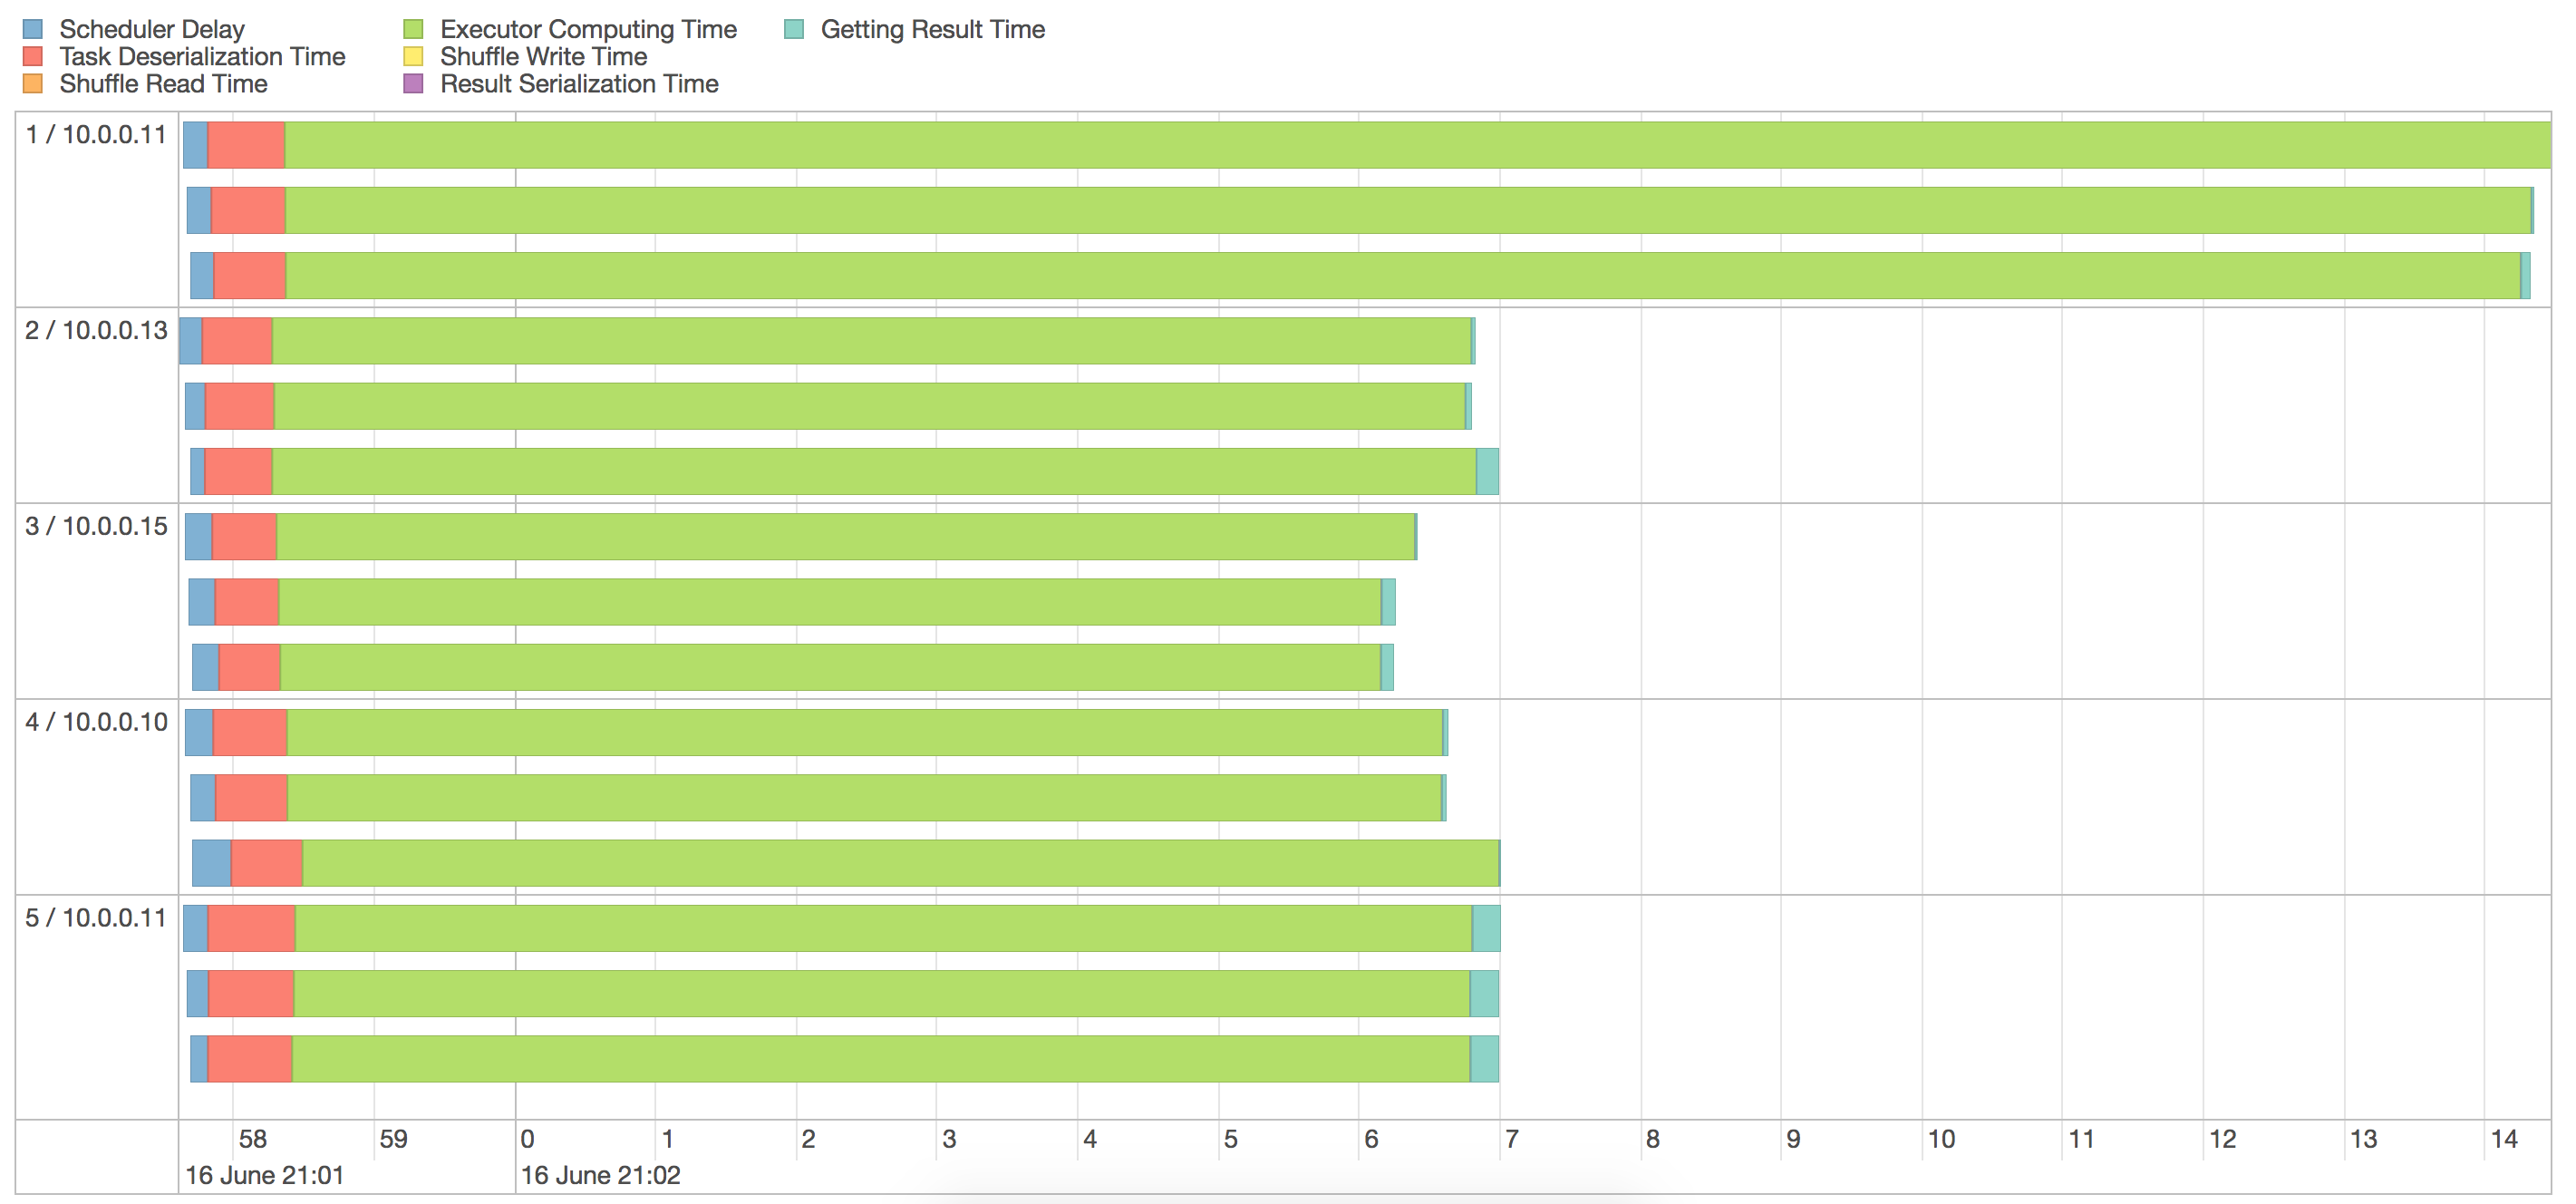
\includegraphics[width=1.0\linewidth]{n2000}
		\caption{Metric with $N=2000$}
		\label{fig:metric:n2000}
	\end{subfigure}
	
	\caption{All metrics to execute into Spark.}
	\label{fig:metric:resumen}
\end{figure}



\section{Conclusion}
\label{sec:results}

OmpCloud is a tool that is very useful for making distributed calculation algorithms without the need to implement a complex system, so any programmer can do it. To use this tool it is necessary to take into account that the number of the calculations to be made must be large, but the resources spent on it, will be spent in vain, this because it can be better to solve the problem in local if the amount of data is low.
\end{document}